%%%%%%%%%%%%%%%%%%%%%%%%%%%%%%%%%%%%%%%%%%%%%%%%%%%%%%%%%%%%%%%%%%%%%%%%%%%%%%%
\chapter{Empuxo} % Sem "Experiência 01" ou qualquer outro número
\label{Chap:ExpEmpuxo}        % para poder trocar a ordem com facilidade
%%%%%%%%%%%%%%%%%%%%%%%%%%%%%%%%%%%%%%%%%%%%%%%%%%%%%%%%%%%%%%%%%%%%%%%%%%%%%%%

\begin{fullwidth}\it
	Realizaremos um experimento para verificar a interação entre um sólido e um fluido quando o primeiro está total ou parcialmente submerso no segundo. Verificaremos experimentalmente o princípio de Arquimedes, calculando através dos dados obtidos a densidade do fluido. Veremos também o conceito de peso aparente e através dele calcularemos a densidade de alguns sólidos. Utilizaremos os seguintes conceitos/técnicas de análise de dados: medidas, algarismos significativos, gráficos, erros de escala e propagados, equação geral para o erro propagado, e regressão linear.
\end{fullwidth}

%%%%%%%%%%%%%%%%%%%%%%%%%%%%%%%%%%%%%%%%%%%%%%%%%%%%%%%%%%%%%%%%%%%%%%%%%%%%%%%
\section{Empuxo}
%%%%%%%%%%%%%%%%%%%%%%%%%%%%%%%%%%%%%%%%%%%%%%%%%%%%%%%%%%%%%%%%%%%%%%%%%%%%%%%

Se tomarmos um bloco de madeira e o colocarmos em uma bacia com água, verificaremos que ele flutua. Sabemos que existe uma força gravitacional que tende a fazer com que o bloco, se pudesse se mover livremente, acelere em direção ao centro da Terra. Concluímos então que a água deve exercer alguma força sobre ele, equilibrando o peso e mantendo o sistema com aceleração nula.

\begin{marginfigure}
\centering
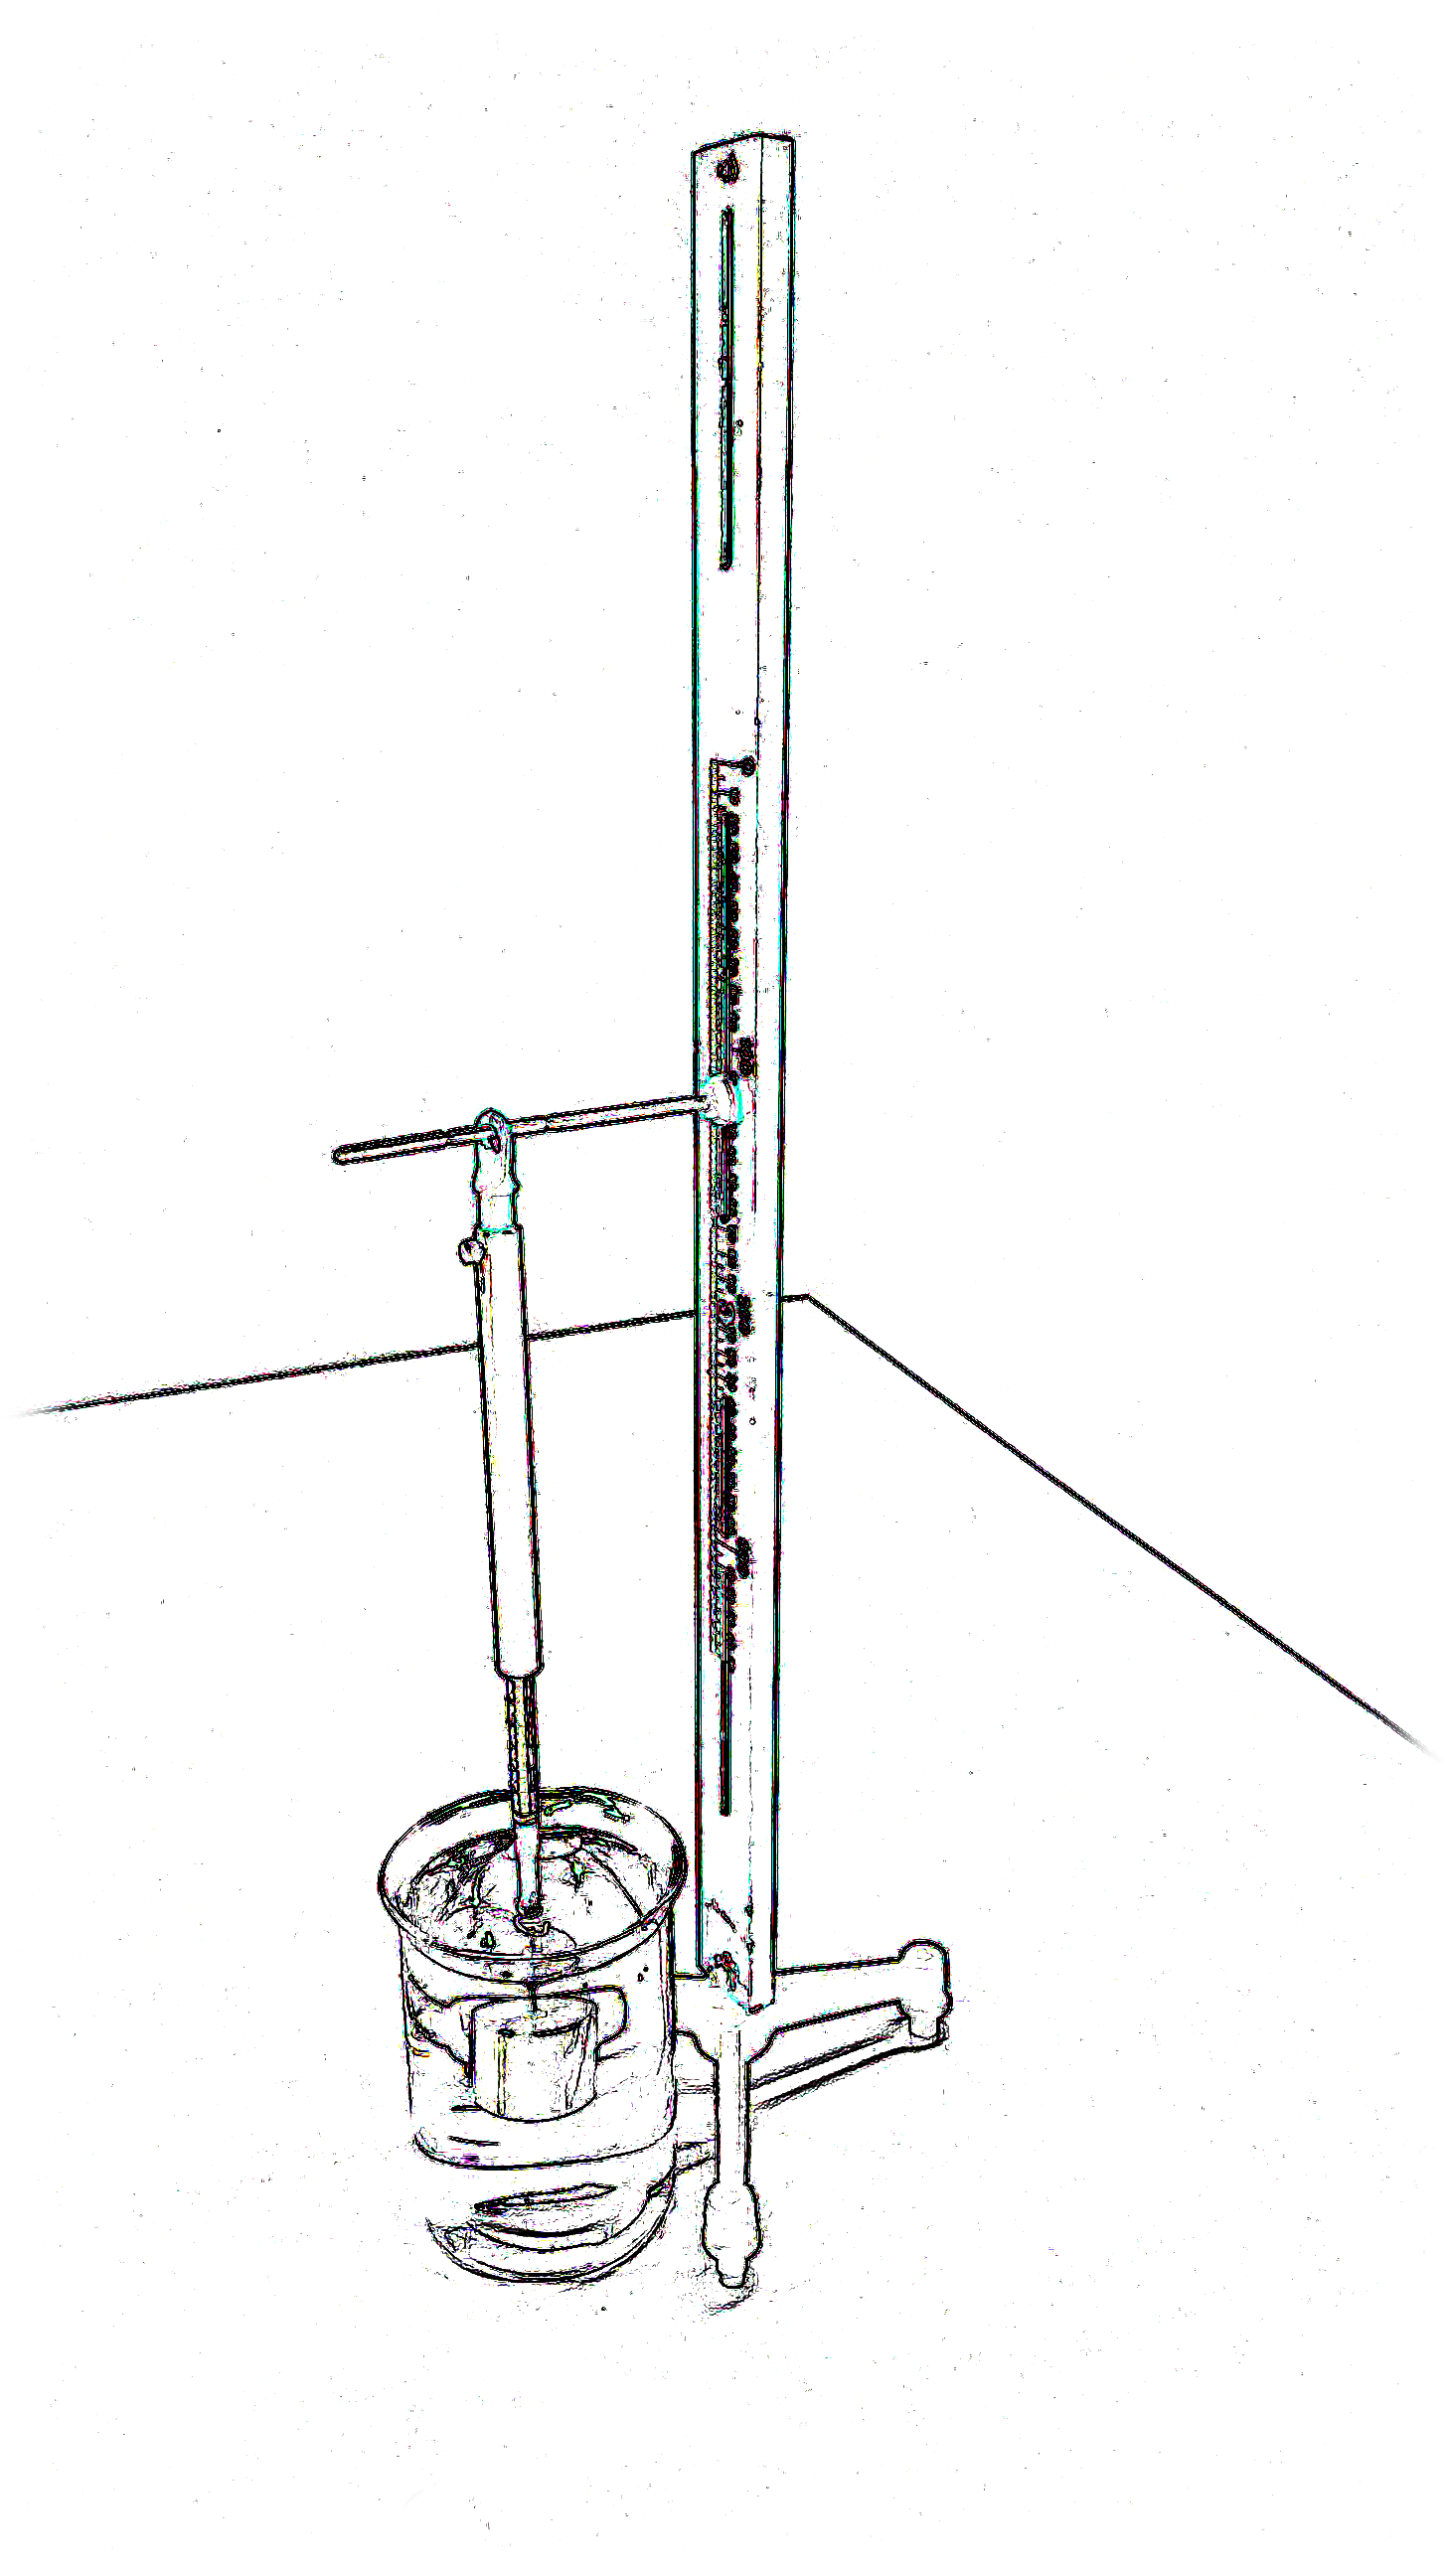
\includegraphics[width=0.7\textwidth]{Ilustrations/Empuxo.png}
\caption{Bloco metálico suspenso por um dinamômetro e submerso em água.}
\label{Fig:BeckerBloco}
\end{marginfigure}

Podemos verificar a origem dessa força se tomarmos um bloco metálico, que afunda ao ser colocado na água e o prendendo a um dinamômetro conforme mostra a Figura~\ref{Fig:BeckerBloco}. Se o becker estiver vazio, claramente a leitura do dinamômetro será igual à força peso do bloco quando o sistema estiver em equilíbrio. Se o enchermos, notaremos que o dinamômetro registrará uma nova medida de força, menor do que a primeira. O valor dessa nova medida é conhecido como \emph{peso aparente} do corpo.

\begin{marginfigure}
\centering
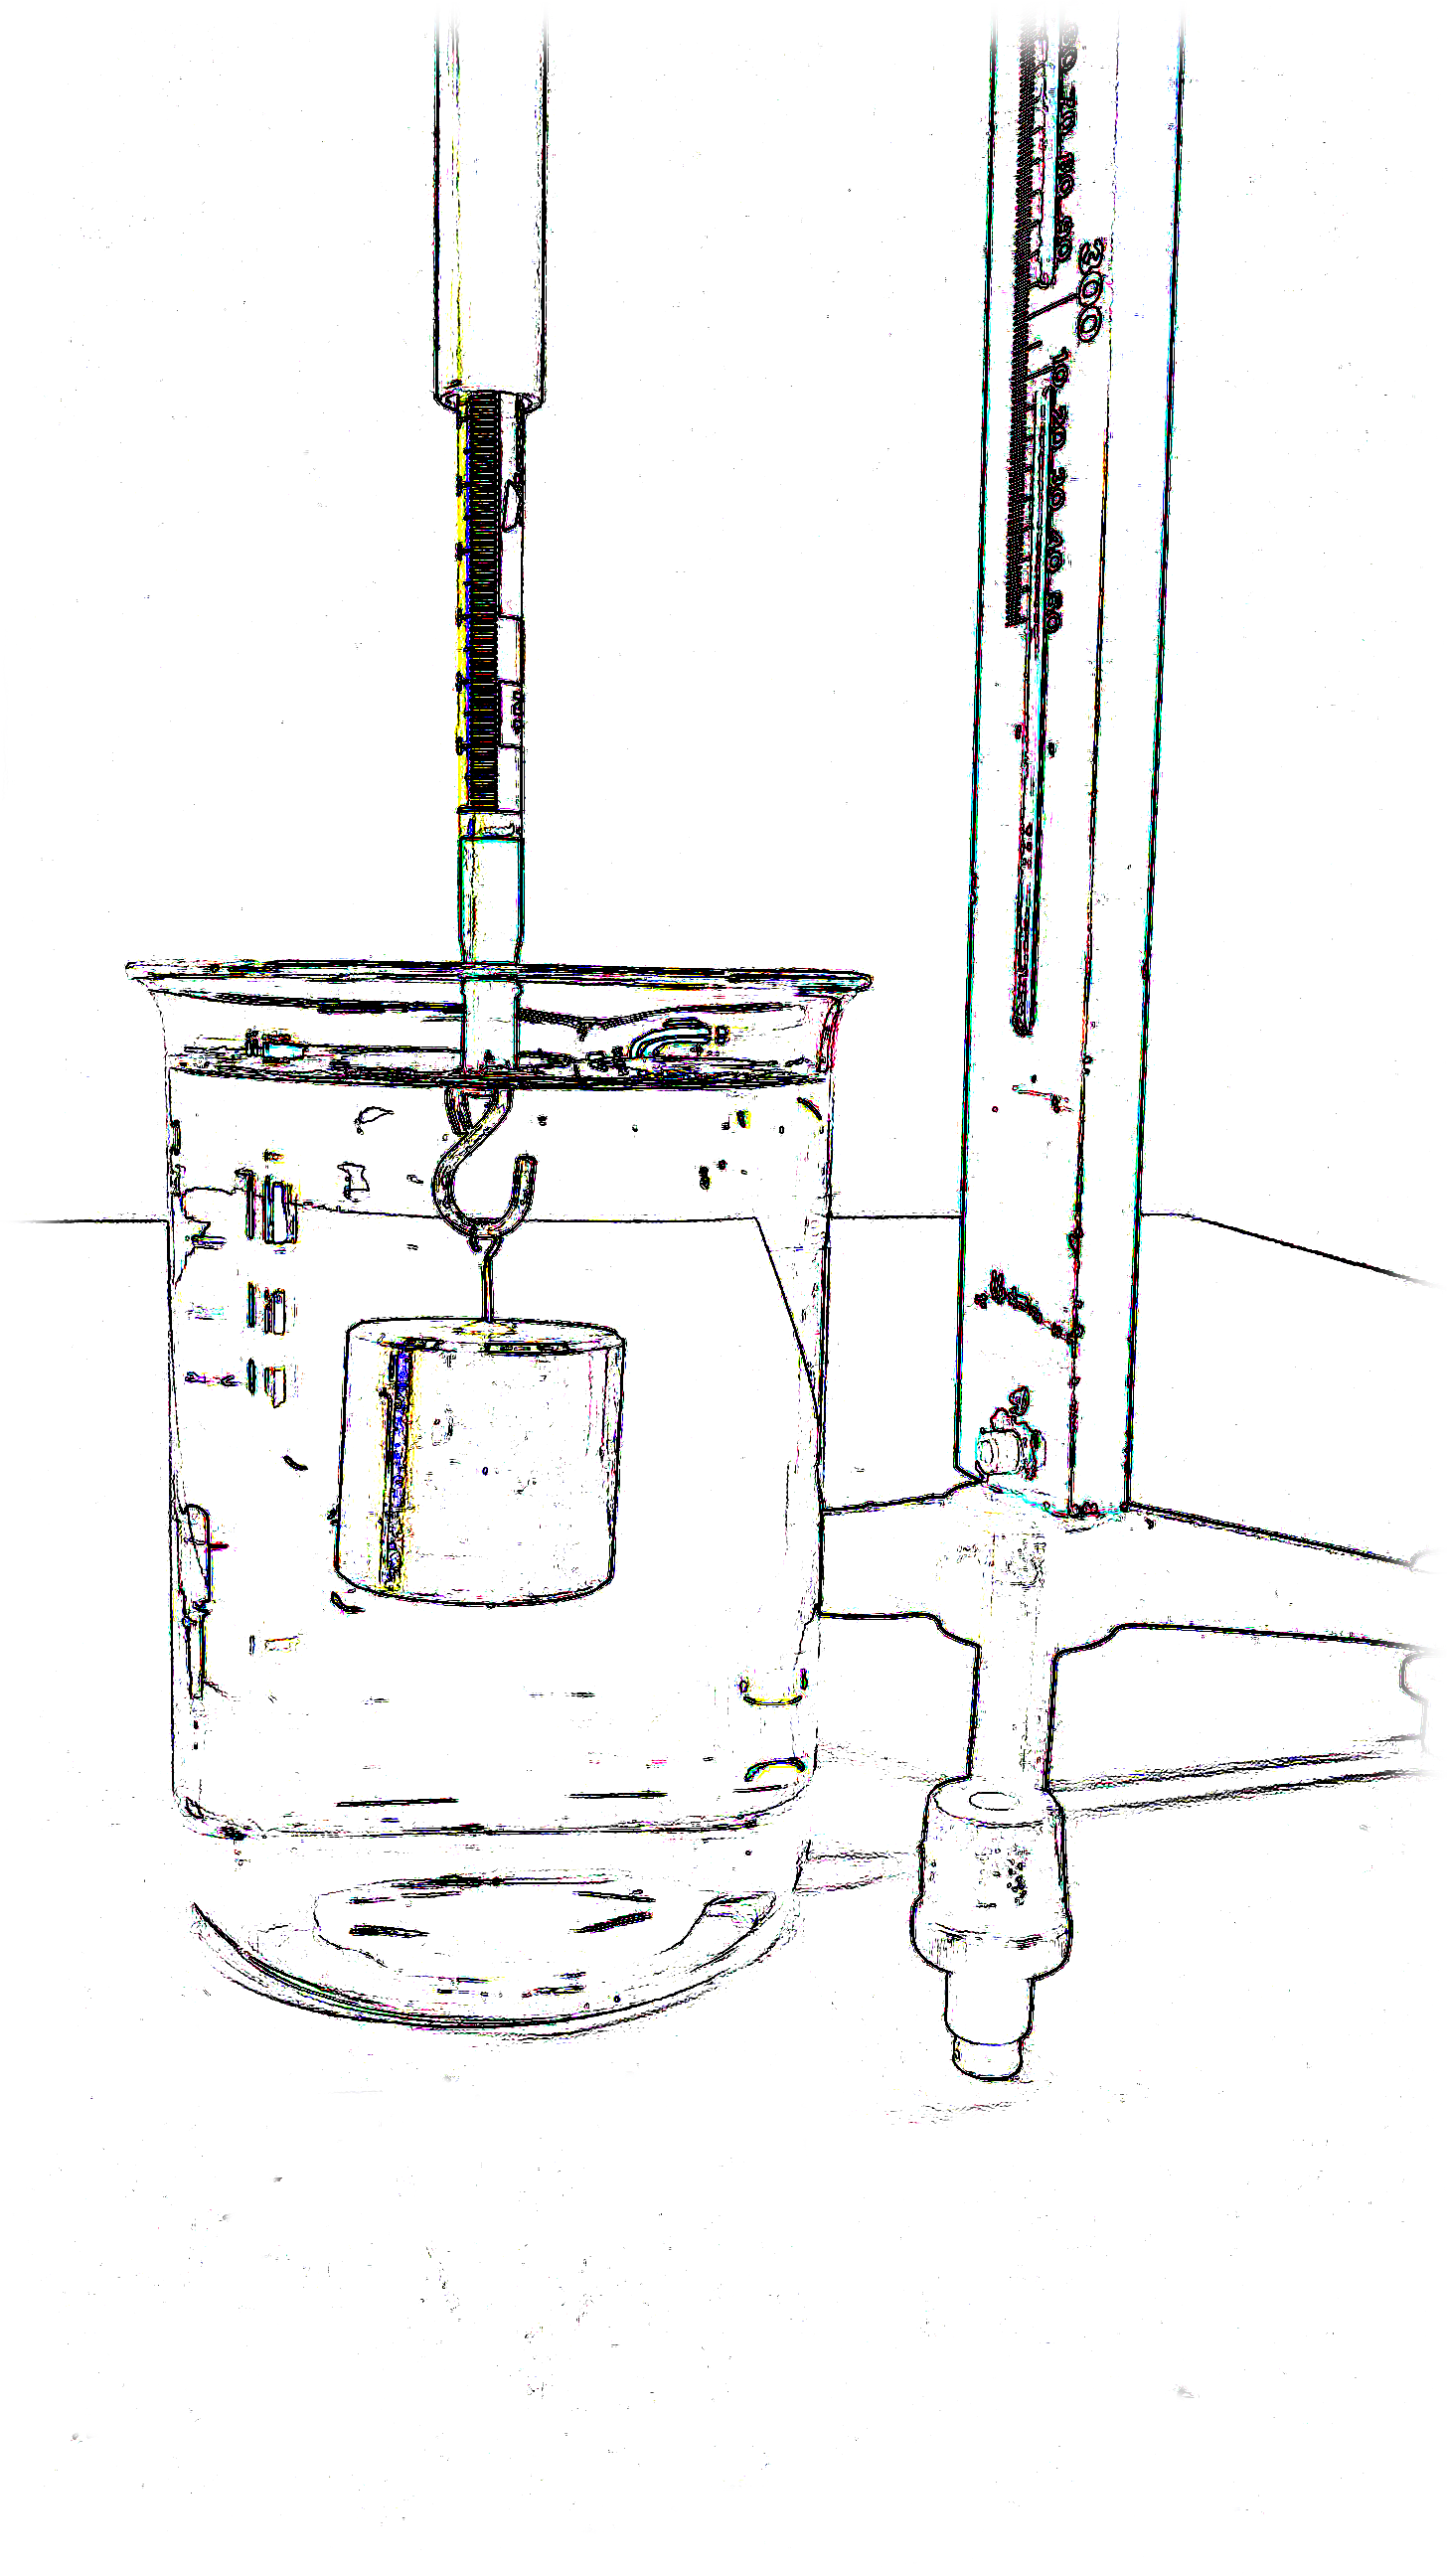
\includegraphics[width=0.5\textwidth]{Ilustrations/Empuxo_detalhe.png}
\caption{Detalhe da Figura~\ref{Fig:BeckerBloco}.}
\label{Fig:BeckerBlocoDetalhe}
\end{marginfigure}
A origem dessa diferença pode ser entendida ao analisarmos as forças exercidas pela pressão do fluido nas superfícies superior e inferior do bloco (as laterais se cancelam). A pressão exercida por um fluido não é constante, aumentando conforme a profundidade aumenta. A pressão é definida como
\begin{equation}
	P = \frac{F}{A},
\end{equation}
%
o que implica em
\begin{equation}
    F = PA.
\end{equation}
%
Logo, a força na parte inferior do bloco é maior que na parte superior, já que as áreas superior e inferior são idênticas. 
\begin{marginfigure}[1cm]
	\centering
	\begin{tikzpicture}[>=Stealth]
		\draw[pattern = north west lines] (0,0) rectangle (1,1);
		\foreach \x in {0,0.333,0.666,1}{
			\draw[->] (\x,-0.75) -- (\x,0);
			\draw[->] (\x,1.25) -- (\x,1);
		}
		\draw[->] (-0.25,1) -- (0,1);
		\draw[->] (-0.375,0.6666) -- (0,0.66666);
		\draw[->] (-0.5625,0.3333) -- (0,0.3333);
		\draw[->] (-0.75,0) -- (0,0);
		\draw[->] (1.25,1) -- (1,1);
		\draw[->] (1.4375,0.6666) -- (1,0.6666);
		\draw[->] (1.625,0.3333) -- (1,0.3333);
		\draw[->] (1.75,0) -- (1,0);
	\end{tikzpicture}
	\caption{Forças atuando nas faces de um bloco submerso.}
	\label{Fig:EmpuxoDiagramaForcas}
\end{marginfigure}

Essa diferença entre as forças é o que denominamos como \emph{força empuxo}, representada aqui como $\vec{F}_e$ (Figura~\ref{Fig:BlocoBeckerDiagrama}). Sua direção e sentido são verticalmente para cima, pois equilibra --- ao menos parcialmente --- o peso. Podemos verificar a intensidade do empuxo  imaginando a seguinte situação: substituímos o volume ocupado pelo bloco por água (veja a Figura~\ref{Fig:BlAguaBeckerDiagrama}). Nesse caso, sabemos que o ``bloco de água'' deve permanecer em equilíbrio, como qualquer outra região do líquido. Se o ``bloco'' está em equilíbrio, seu peso está sendo equilibrado pelo empuxo. Logo, \emph{o empuxo tem o mesmo módulo que o peso do líquido deslocado}\footnote{Este resultado é conhecido como \emph{princípio de Arquimedes}.}. No caso do bloco metálico acima, o empuxo é equivalente ao peso de um ``bloco de água'' com o mesmo volume que o bloco metálico.

\begin{marginfigure}
\centering
\begin{tikzpicture}[>=Stealth]
	\draw[color=gray] (-1,-1) rectangle (2,2);
	\draw (0,0) rectangle (1,1);
	\foreach \x in {0,0.333,0.666,1}{
			\draw[->] (\x,-0.75) -- (\x,0);
			\draw[->] (\x,1.25) -- (\x,1);
	}
	\draw (1,1.125) node[anchor=west]{$\vec{F}_{\textrm{sup}}$};
	\draw (1,-0.675) node[anchor=west]{$\vec{F}_{\textrm{inf}}$};
	\draw[->] (0.5,0.5) -- node[above right] {$\vec{P}$} (0.5,-0.5);
	\draw[fill] (0.5,0.5) circle (0.02);	

	\draw[->] (2.5,0.5) -- (2.5,1.25) node[anchor=west]{$\vec{F}_{\textrm{inf}}$};
	\draw[->] (2.5,0.5) -- (2.5,0.25) node[anchor=west]{$\vec{F}_{\textrm{sup}}$};
	\draw[->] (2.5,0.5) -- (2.5,-0.5) node[anchor=west] {$\vec{P}$};
	\draw[fill] (2.5,0.5) circle (0.02);
	
	\draw[fill] (3.5,0.5) circle (0.02);
	\draw[->] (3.5,0.5) -- (3.5,-0.5) node[anchor=west] {$\vec{P}$};
	\draw[->] (3.5,0.5) -- (3.5,1) node[anchor=west]{$\vec{F}_{e}$};
\end{tikzpicture}
\caption{Diagrama de corpo livre representando as forças que atuam sobre o bloco quando submerso. No diagrama à direita, substituímos a soma $\vec{F}_{\textrm{inf}} + \vec{F}_{\textrm{sup}}$ das forças que atuam na parte inferior e superior do bloco por $F_e$, isto é, o empuxo. As forças laterais não estão representadas pois, por simetria, se equilibram.}
\label{Fig:BlocoBeckerDiagrama}
\end{marginfigure}

\begin{marginfigure}
\centering
\begin{tikzpicture}[>=Stealth]
	\draw[color=gray] (-1,-1) rectangle (2,2);
	\draw[dashed] (0,0) rectangle (1,1);
	\foreach \x in {0,0.333,0.666,1}{
			\draw[->] (\x,-0.75) -- (\x,0);
			\draw[->] (\x,1.25) -- (\x,1);
	}
	\draw (1,1.125) node[anchor=west]{$\vec{F}_{\textrm{sup}}$};
	\draw (1,-0.675) node[anchor=west]{$\vec{F}_{\textrm{inf}}$};
	\draw[->] (0.5,0.5) -- node[right] {$\vec{P}$} (0.5,0);
	\draw[fill] (0.5,0.5) circle (0.02);	

	\draw[->] (2.5,0.5) -- (2.5,1.25) node[anchor=west]{$\vec{F}_{\textrm{inf}}$};
	\draw[->] (2.5,0.5) -- (2.5,0.25) node[anchor=west]{$\vec{F}_{\textrm{sup}}$};
	\draw[->] (2.5,0.5) -- (2.5,0) node[anchor=east] {$\vec{P}$};
	\draw[fill] (2.5,0.5) circle (0.02);
	
	\draw[fill] (3.5,0.5) circle (0.02);
	\draw[->] (3.5,0.5) -- (3.5,0) node[anchor=west] {$\vec{P}$};
	\draw[->] (3.5,0.5) -- (3.5,1) node[anchor=west]{$\vec{F}_{e}$};
\end{tikzpicture}
\caption{Diagrama de corpo livre representando as forças que atuam sobre uma massa de água que ocupa o volume original do bloco. As forças devido à pressão são iguais ao caso do bloco, porém o peso é menor. Como o meio é todo composto por água e deve então estar em equilíbrio, concluímos que o empuxo deve ser igual ao peso do volume de água deslocado (caso contrário não haveria equilíbrio).}
\label{Fig:BlAguaBeckerDiagrama}
\end{marginfigure}
%%%%%%%%%%%%%%%%%%%%%%%%%%%%%%%%%%%%%%%%%%%%%%%%%%%%%%%%%%%%%%%%%%%%%%%%%%%%%%%
\section{Cálculo de densidades}
%%%%%%%%%%%%%%%%%%%%%%%%%%%%%%%%%%%%%%%%%%%%%%%%%%%%%%%%%%%%%%%%%%%%%%%%%%%%%%%

%%%%%%%%%%%%%%%%%%%%%%%%%%%%%%%%%%%
\subsection{Densidade de um sólido}
%%%%%%%%%%%%%%%%%%%%%%%%%%%%%%%%%%%

Podemos calcular a razão da densidade de um objeto pela densidade da água usando um dinamômetro e uma proveta. Se pendurarmos o objeto no dinamômetro, verificaremos que --- no equilíbrio --- ele nos dará a leitura do módulo da força peso do objeto. Quando o mergulhamos, no entanto, teremos uma leitura menor, que denominamos anteriormente como peso aparente.

Temos então que
\begin{align}
	P &= \rho Vg \\
	F_E &= \rho_{\textrm{água}} V g
\end{align}
%
onde $E$ é igual ao peso do volume de água deslocado, $\rho$ é a densidade do material e $\rho_{\textrm{água}}$ é a densidade da água. Calculando a razão entre as equações acima, temos
\begin{equation}
	\frac{P}{F_E} = \frac{\rho Vg}{\rho_{\textrm{água}}Vg} = \frac{\rho}{\rho_{\textrm{água}}},
\end{equation}
%
de onde podemos escrever, lembrando que o peso aparente é dado por
\begin{equation}
	P_{\textrm{ap}} = P - F_E,
\end{equation}
%
a seguinte relação para a razão $\rho/\rho_{\textrm{água}}$:
\begin{equation}\label{Eq:DensRelativa}
	\frac{\rho}{\rho_{\textrm{água}}} = \frac{P}{P-P_{\textrm{ap}}}.
\end{equation}

%%%%%%%%%%%%%%%%%%%%%%%%%%%%%%%%%%%
\subsection{Densidade de um fluido}
%%%%%%%%%%%%%%%%%%%%%%%%%%%%%%%%%%%

Podemos utilizar uma proveta, um fluido, uma balança, e um conjunto de corpos de prova para verificar a densidade e um corpo de prova para verificar a densidade do fluido.


\begin{marginfigure}
\centering
\begin{tikzpicture}[>=Stealth,
     interface/.style={
        % superfície
        postaction={draw,decorate,decoration={border,angle=-45,
                    amplitude=0.2cm,segment length=2mm}}},
    ]

    \draw[interface] (-2,0) -- (2,0);
    
    \draw[pattern = north west lines] (-1.5,3) -- (-1.5,0) -- (1.5,0) -- (1.5,3) -- (1.3,3) -- (1.3,0.2) -- (-1.3, 0.2) -- (-1.3,3) -- cycle;
    
    %\draw[pattern = dots] (-1.3,2.5) -- (0,2.5) -- (0,2) -- (-0.5,2) -- (-0.5, 1) -- (0.5,1) -- (0.5,2) -- (0,2) -- (0,2.5) -- (1.3,2.5) -- (1.3,0.2) -- (-1.3,0.2) -- cycle;
    
    \draw[dashed] (-1.3, 2.75) -- (1.3, 2.75);
        
    \draw (0,2) -- (0,4);
    \draw[->, thick] (0,2) -- (0,3.25) node[right]{$\vec{T}$};
    \draw[pattern = north west lines] (-0.5,1) rectangle (0.5,2);
    
    \draw[->, thick] (-0.25,2) -- +(0,0.5) node[left]{$\vec{E}$};
    \draw[<-, thick] (-0.25,0.2) -- node[left]{$\vec{E}'$} +(0,0.5);
    
\end{tikzpicture}
\caption{A reação à força de empuxo exercida sobre o corpo atua sobre o fundo do recipiente.\label{Fig:ReacaoEmpuxo}}
\end{marginfigure}

Se tomarmos a proveta e a preenchermos com água até um certo nível, podemos pesá-la e encontraremos um valor para a massa do sistema. Ao pendurarmos o corpo de prova de forma que ele \emph{esteja submerso, porém sem tocar as laterais da proveta ou seu fundo}, verificaremos um aumento na leitura da balança, porém esse aumento \emph{não corresponderá à massa do corpo}. Ao verificarmos o diagrama de forças das Figuras~\ref{Fig:BlocoBeckerDiagrama} e~\ref{Fig:BlAguaBeckerDiagrama}, vemos que ao mergulharmos o corpo, há uma força de empuxo $\vec{E}$ dirigida para cima e que equilibra parcialmente o peso do objeto. Onde está a reação a esta força de empuxo? A reação a esta força deve agir sobre o líquido, que --- por sua vez --- exerce força sobre as paredes do recipiente (Figura~\ref{Fig:ReacaoEmpuxo}). Como as forças exercidas sobre uma lateral qualquer se equilibram com as forças exercidas sobre a lateral oposta, resta a força exercida sobre o fundo do recipiente. Nessa situação, temos então que a balança registrará uma ``massa aparente'' adicional dada por\footnote{Mesmo em uma balança de braços, o que a balança registra é a força normal exercida para equilibrar o objeto, apesar de a escala estar marcada em unidades de massa.}
\begin{equation}
	m_{\textrm{ap}} = \frac{F_E}{g}.
\end{equation}
%
Como o empuxo é o peso do volume de água deslocado, temos
\begin{align}
	m_{\textrm{ap}} &= \frac{m_{\textrm{água}}g}{g} \\
	&=m_{\textrm{água}}.
\end{align}
%
Podemos então calcular a densidade da água através da razão entre a diferença das massas (depois e antes da submersão do corpo) e a diferença dos volumes indicados pela proveta:\footnote{As variáveis $m'$ e $V'$ denotam os valores registrados pela balança e pela proveta após a submersão do corpo.}
\begin{equation}
	\rho_{\textrm{água}} = \frac{m'-m}{V'-V}.
\end{equation}

Note que se tomarmos um gráfico dos valores de $m'\times V'$ para diversos corpos submersos, temos que a inclinação do gráfico será dada por
\begin{equation}
    B = \frac{\Delta m}{\Delta V}.
\end{equation}
%
Assim, se fizermos um gráfico desse tipo e traçarmos a melhor reta, podemos obter $\rho_{\text{água}}$ através do coeficiente angular. 


%%%%%%%%%%%%%%%%%%%%%%%%%%%%%%%%%%%%%%%%%%%%%%%%%%%%%%%%%%%%%%%%%%%%%%%%%%%%%%%
\section{Experimento}
%%%%%%%%%%%%%%%%%%%%%%%%%%%%%%%%%%%%%%%%%%%%%%%%%%%%%%%%%%%%%%%%%%%%%%%%%%%%%%%

%%%%%%%%%%%%%%%%%%%%%%
\subsection{Objetivos}
\label{Sec:ObjetivosEmpuxo}
%%%%%%%%%%%%%%%%%%%%%%

\begin{itemize}
	\item Verificar experimentalmente a existência da força de empuxo e a existência de um peso aparente para um objeto submerso.
	\item Verificar experimentalmente a densidade de corpos de prova utilizando um dinamômetro e uma proveta.
	\item Verificar experimentalmente a reação ao empuxo.
	\item Verificar experimentalmente a densidade de um líquido utilizando uma balança e uma proveta.
\end{itemize}

%%%%%%%%%%%%%%%%%%%%%%%%%%%%%%%%%%%%%%%%%%%%%%%%%%%%%%%%%%%%%%%%%%%%%%%%%%%%%%%
\section{Material Necessário}
%%%%%%%%%%%%%%%%%%%%%%%%%%%%%%%%%%%%%%%%%%%%%%%%%%%%%%%%%%%%%%%%%%%%%%%%%%%%%%%

\begin{itemize}
	\item Proveta;
	\item Balança;
	\item Dinamômetro;
	\item Becker com água;
	\item Corpos de prova diversos;
	\item Suporte vertical com haste horizontal.
\end{itemize}

%%%%%%%%%%%%%%%%%%%%%%%%%%%%%%%%%%%%%%%%%%%%%%%%%%%%%%%%%%%%%%%%%%%%%%%%%%%%%%%
\section{Procedimento Experimental}
%%%%%%%%%%%%%%%%%%%%%%%%%%%%%%%%%%%%%%%%%%%%%%%%%%%%%%%%%%%%%%%%%%%%%%%%%%%%%%%

%%%%%%%%%%%%%%%%%%%%%%%%%%%%%%%%%%%%%%%%%%%%%%%%%%%
\subsection{Determinação da densidade de um sólido}
%%%%%%%%%%%%%%%%%%%%%%%%%%%%%%%%%%%%%%%%%%%%%%%%%%%
\begin{enumerate}
	\item Disponha o dinamômetro na vertical com o auxílio do suporte com haste.
	\item Zere o dinamômetro
	\item Suspenda um corpo de prova usando o gancho do dinamômetro e efetue a leitura do peso real.
	\item Mergulhe o corpo de prova de forma que ele não toque nas paredes e no fundo do becker. Verifique o valor do peso aparente.
	\item Anote os dados obtidos para o peso na Tabela~\ref{Tab:DadosEmpuxo}
	\item Repita os itens 3 a 5 acima para os demais corpos de prova.
\end{enumerate}

%%%%%%%%%%%%%%%%%%%%%%%%%%%%%%%%%%%%%%%%%%%%%%%%%
\subsection{Determinação da densidade da água}
%%%%%%%%%%%%%%%%%%%%%%%%%%%%%%%%%%%%%%%%%%%%%%%%%
\begin{enumerate}
\item Coloque \np[ml]{150,0} na proveta e meça a massa da proveta com a água;
\item Mergulhe o corpo de prova na proveta, cuidando para que ele não toque no fundo e nas bordas da proveta e determine a massa do conjunto;
\item Obtenha também a leitura para o volume indicado pela proveta.
\item Repita os itens 2 e 3 para os demais corpos.
\item Anote os resultados na Tabela~\ref{Tab:DadosEmpuxo}
\end{enumerate}

%%%%%%%%%%%%%%%%%%%%%%%%%%%%%%%%%%%%%%%%%%%%%%%%%%%%%%%%%%%%%%%%%%%%%%%%%%%%%%%
%%%%%%%%%%%%%%%%%%%%%%%%%%%%%%%%%%%%%%%%%%%%%%%%%%%%%%%%%%%%%%%%%%%%%%%%%%%%%%%
%%%%%%%%%%%%%%%%%%%%%%%%%%%%%%%%%%%%%%%%%%%%%%%%%%%%%%%%%%%%%%%%%%%%%%%%%%%%%%%
%%%%%%%%%%%%%%%%%%%%%%%%%%%%%%%%%%%%%%%%%%%%%%%%%%%%%%%%%%%%%%%%%%%%%%%%%%%%%%%
\cleardoublepage

\noindent{}{\huge\textit{Empuxo}}

\vspace{15mm}

\begin{fullwidth}
\noindent{}\makebox[0.6\linewidth]{Turma:\enspace\hrulefill}\makebox[0.4\textwidth]{  Data:\enspace\hrulefill}
\vspace{5mm}

\noindent{}\makebox[0.6\linewidth]{Aluno(a):\enspace\hrulefill}\makebox[0.4\textwidth]{  Matrícula:\enspace\hrulefill}

\noindent{}\makebox[0.6\linewidth]{Aluno(a):\enspace\hrulefill}\makebox[0.4\textwidth]{  Matrícula:\enspace\hrulefill}

\noindent{}\makebox[0.6\linewidth]{Aluno(a):\enspace\hrulefill}\makebox[0.4\textwidth]{  Matrícula:\enspace\hrulefill}

\noindent{}\makebox[0.6\linewidth]{Aluno(a):\enspace\hrulefill}\makebox[0.4\textwidth]{  Matrícula:\enspace\hrulefill}

\noindent{}\makebox[0.6\linewidth]{Aluno(a):\enspace\hrulefill}\makebox[0.4\textwidth]{  Matrícula:\enspace\hrulefill}
\end{fullwidth}

\vspace{5mm}

%%%%%%%%%%%%%%%%%%%%%%%%%%%%%%%%%%%%%%%%%%%%%%%%%%%%%%%%%%%%%%%%%%%%%%%%%%%%%%%
\section{Questionário}
%%%%%%%%%%%%%%%%%%%%%%%%%%%%%%%%%%%%%%%%%%%%%%%%%%%%%%%%%%%%%%%%%%%%%%%%%%%%%%%

\begin{question}[type={exam}]{1}
Apresente os resultados de maneira clara e organizada. Mostre os cálculos requisitados de maneira clara e sucinta, evidenciando o raciocínio desenvolvido.
\end{question}

\begin{question}[type={exam}]{1}
Liste os equipamentos utilizados. Para os instrumentos de medida, descreva o tipo do equipamento, sua resolução, e seu erro de escala.
\end{question}

\begin{question}[type={exam}]{1}
Preencha as tabelas com o número adequado de algarismos significativos, unidades, e erros de escala apropriados. 
\end{question}

\begin{question}[type={exam}]{1}
Elabore um gráfico de $m' \times V'$ para os dados da Tabela~\ref{Tab:DadosEmpuxo}.
\end{question}

\begin{question}[type={exam}]{1.5}
Calcule a reta que melhor representa os dados experimentais na questão acima utilizando o método dos mínimos quadrados e a adicione ao gráfico.
\end{question}

\begin{question}[type={exam}]{1.5}
Calcule os valores para a densidade relativa $(\rho/\rho_{\textrm{água}})$ dos sólidos, juntamente com o erro propagado, através da Equação~\ref{Eq:DensRelativa}. Preencha a coluna correspondente da Tabela~\ref{Tab:DadosEmpuxo}. 
\end{question}

\begin{question}[type={exam}]{1.5}
Deduza a equação para o erro em uma divisão
\begin{equation}
    (q \pm \delta q) = (x \pm \delta x) \div (y \pm \delta y)
\end{equation}
%
a partir da Equação~\eqref{Eq:ErroGeral}.
\end{question}

\begin{question}[type={exam}]{1.5}
Considerando os objetivos do experimento, listados na Seção~\ref{Sec:ObjetivosEmpuxo}, e os resultados obtidos nas questões anteriores, discuta quais objetivos foram atingidos com sucesso, justificando suas conclusões. Se algum objetivo não foi atingido, discuta quais são os possíveis motivos do fracasso e que providências podem ser tomadas para que eles sejam alcançados.
\end{question}

\vfill
%%%%%%%%%%%%%%%%%%%%%%%%%%%%%%%%%%%%%%%%%%%%%%%%%%%%%%%%%%%%%%%%%%%%%%%%%%%%%%%
\pagebreak
\section{Tabelas}
%%%%%%%%%%%%%%%%%%%%%%%%%%%%%%%%%%%%%%%%%%%%%%%%%%%%%%%%%%%%%%%%%%%%%%%%%%%%%%%

\begin{table}
\label{Tab:DadosEmpuxo}
	\begin{center}
		\begin{tabular}{cp{25mm}p{25mm}p{25mm}c}
		\toprule
		&\multicolumn{3}{l}{\textbf{Dados de peso e peso aparente para os corpos de prova.}} \\
		\cmidrule{2-4}
		& $P$ & $P_{\textrm{ap}}$ & $\rho/\rho_{\textrm{água}}$ & \\
		\cmidrule{2-4}
		& \cellcolor[gray]{0.89} & \cellcolor[gray]{0.92} & \cellcolor[gray]{0.89} \\
		& \cellcolor[gray]{0.95} & \cellcolor[gray]{0.97} & \cellcolor[gray]{0.95} \\
		& \cellcolor[gray]{0.89} & \cellcolor[gray]{0.92} & \cellcolor[gray]{0.89} \\
		& \cellcolor[gray]{0.95} & \cellcolor[gray]{0.97} & \cellcolor[gray]{0.95} \\
		& \cellcolor[gray]{0.89} & \cellcolor[gray]{0.92} & \cellcolor[gray]{0.89} \\
\\
		&\multicolumn{3}{l}{\textbf{Dados a leitura de volume e massa.}} \\
		\cmidrule{2-3}
		& $V'$ & $m'$ \\
		\cmidrule{2-3}
		& \cellcolor[gray]{0.89} & \cellcolor[gray]{0.92} \\
		& \cellcolor[gray]{0.95} & \cellcolor[gray]{0.97} \\
		& \cellcolor[gray]{0.89} & \cellcolor[gray]{0.92} \\
		& \cellcolor[gray]{0.95} & \cellcolor[gray]{0.97} \\
		& \cellcolor[gray]{0.89} & \cellcolor[gray]{0.92} \\
		\cmidrule{2-3}
		\cmidrule{2-4}
		\bottomrule
		\end{tabular}
	\end{center}
	\caption{Dados para as leituras de massa, volume, peso e peso aparente.}
\end{table}
%
